\section{Desenvolvimento}

Iremos nos aprofundar no desenvolvimento destes autômatos. <expandir>

\subsection{Máquina de Estado Finito}

<falar sobre memória>

Uma máquina de estado finito (MEF) pode ser considerada como um modelo
simplificado do funcionamento de um computador. Esta pode ser definida como uma
quíntupla ordenada $M = (S, I, O, f_S, f_O)$ onde:
\begin{itemize}
    \item $S$ é o conjunto finito de estados;
    \item $I$ é o conjunto finito de símbolos de entrada (alfabeto de entrada);
    \item $O$ é o conjunto finito de símbolos de saída (alfabeto de saída);
    \item $f_S: S \times I \rightarrow S$ é uma função que retorna o próximo
          estado $s_{t_{k+1}} \in S$ dado o estado anterior $s_{t_k} \in S$ e
          um símbolo de entrada $i_{t_k} \in I$;
    \item $f_O: S \rightarrow O$ é a função \textit{output}, que retorna o
          símbolo de saída $o_{t_k} \in O$ do estado atual $s_{t_k} \in S$.
\end{itemize}

As operações da MEF são sincronizadas por pulsos discretos de um relógio
(\emph{clock}) representados por $t_k$, onde $k \in \mathbb{N}_0$ representa o
ciclo de \textit{clock} atual. Partindo de um estado inicial $s_0 = s_{t_0}$,
após um pulso de \textit{clock}, a função $f_S$ retornará um novo estado
$s_{t_1}$ dado a entrada anterior $i_{t_0}$ e o estado anterior $s_0$.
Generalizando para qualquer pulso de \textit{clock}, é possível afirmar que a
MEF possui um comportamento determinístico, ou seja, o novo estado sempre
dependará do estado e entrada anteriores. Para cada um dos estados, há um
símbolo de saída, que é retornado pela função \textit{output} $f_O$.

\begin{figure}[H]
    \centering
    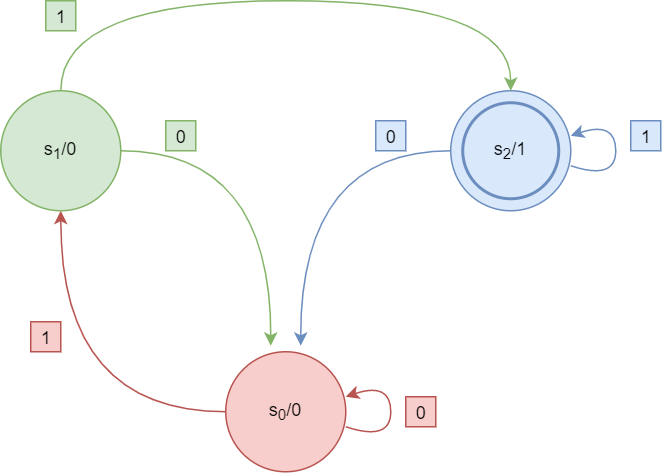
\includegraphics[width=0.7\textwidth]{fsm}
    \caption{Exemplo de máquina de estado finito}
\end{figure}

Tomando como exemplo a MEF acima, começamos no estado $s_0$ e temos como saída o
símbolo \textbf{0}. Aqui, há duas possibilidades: enquanto a entrada for
\textbf{0}, permanecemos neste estado; caso a entrada seja \textbf{1}, seguimos
para o estado $s_1$. Ao seguirmos para o estado $s_1$ temos como saída o símbolo
\textbf{0}. Novamente, há duas possíveis entradas: caso a entrada seja
\textbf{0}, retornamos ao estado $s_0$; caso a entrada seja \textbf{1}, seguimos
para o estado $s_2$. Por fim, ao seguirmos para o estado $s_2$ temos como saída
o símbolo \textbf{1}. As alternativas são: caso a entrada seja \textbf{0},
retornarmos ao estado $s_0$; enquanto a entrada seja \textbf{1}, permanecemos
neste estado.

Esta forma um tanto verbosa de se descrever uma MEF pode ser colocada em uma
tabela, com o estado atual, possíveis entradas e saídas como colunas da mesma.

\begin{center}
    % https://tex.stackexchange.com
    % /questions/192842/multiple-columns-in-table-problem-with-alignment
    % Use `L{width}', `C{width}' or `R{width}' for column alignment
    \begin{tabular}{ c C{1cm} C{1cm} c }
        \toprule
        Estado Atual & \multicolumn{2}{c}{Próximo Estado} & Saída  \\
                     & \textbf{0} & \textbf{1} &                   \\
        \hline
        $s_0$        & $s_0$      & $s_1$      & \textbf{0}        \\
        $s_1$        & $s_0$      & $s_2$      & \textbf{0}        \\
        $s_2$        & $s_0$      & $s_2$      & \textbf{1}        \\
        \bottomrule
    \end{tabular}
\end{center}

Nota-se que dentre todas as possíveis entradas, esta MEF só aceitará, isto é,
terminará no estado final $s_2$, para \emph{strings} de entrada que terminem
com dois ou mais \textbf{1} (\textbf{11}, \textbf{111}, \textbf{1111}, \ldots).

\subsection{Máquina de Turing}

<expandir>